\documentclass[12pt]{report}
\usepackage{commands}

\begin{document}

\large
\begin{center}
AMSC 660 Homework 4\\
Due Sep 27\\
By Marvyn Bailly\\
\end{center}
\normalsize
\hrule



\newtheorem{theorem}{Theorem}

%Good luck my man
%---------------%
%---Problem 1---%
%---------------%


\begin{problem}%[vskip]
\subsection*{Problem 1}

Read Sections 4.1-4.3 on Ky-Fan norms and low-rank approximations based on SVD in LinearAlgebra.pdf. Prove the Eckart-Young-Mirsky theorem for any Ky-Fan norm.

\begin{theorem}
    Let $A = U\Sigma V^T$ be an SVD of $A$ and $M$ be any matrix of the size of $A$ such that $\text{rank}(M) \leq k$. Then
    \[
         \|A - M \| \geq \|A - U_k\Sigma_k V_k^T \|,
    \]
    for any Ky-Fan norm $\| \cdot \|$, where $U_k$ and $V_k$ consist of the first $k$ columns of $U$ and $V$, respectively and $\sigma_k = \text{diag}(\sigma_1,\cdots,\sigma_k)$. 
\end{theorem}

\noindent You can use Lemma 1 in Section 4.3 in LinearAlgebra.pdf.

\subsection*{Solution}
\begin{proof}

Let $A = U \Sigma V^T$ be the SVD of $A \in \R^{n\times d}$ and let $M \in \R^{n \times d}$ such that $\text{rank}(M) \leq k$. From Lemma 1,
\begin{equation}\label{eq1}
    \sigma_{k+i}(A) \leq \sigma_i(A-M) + \sigma_{k+1}(M) = \sigma_i(A-M),
\end{equation}
where $\sigma_{k+1}(M) = 0$ since the $\text{rank}(M) \leq k$. Recalling that Ky-Fan norms are $l^p$ norms of the vector of singular value, let $\| \cdot \|_p$ denote the $p$ Ky-Fan norm and observe
\begin{align*}
    \|A - M\|_p^p &= \sum_{i=1}^d\sigma_i(A-m)^p\\
                &\geq \sum_{i=1}^{d-k}\sigma_{k+i}(A)^p ~~(\text{by Eq. \ref{eq1}})\\
                &= \sum_{j=k+1}^d \sigma_j(A)^p.
\end{align*} 
Thus $\|A - M\|_p \geq \paren{\sum_{j=k+1}^d \sigma_j(A)^p}^{1/p}.$ Now noticing that $A = \sum_{i=1}^d u_i \sigma_i v_i^T$ and $A_k = \sum_{i=1}^k u_i \sigma_i v_i^T$. Then 
\[
    \left\|A - U_k\Sigma_k V_l^T\right\|_p = \left\| \sum_{i=1}^d u_i \sigma_i v_i^T - \sum_{i=1}^k u_i \sigma_i v_i^T\right\|_p = \left\|\sum_{i=k+1}^d u_i \sigma_i v_i^T\right\|_p = \left( \sum_{i=k+1}^d \sigma_i(A)^p \right)^{1/p}.
\]
Therefore
\[
    \|A - M\|_p \geq \paren{\sum_{j=k+1}^d \sigma_j(A)^p}^{1/p} = \left\|A - U_k\Sigma_k V_l^T\right\|_p.
\]


\end{proof}
\end{problem}




%---------------%
%---Problem 2---%
%---------------%


\begin{problem}%[vskip]
\subsection*{Problem 2}

Find an upper bound for the condition number for eigenvector $r_J$ of a non-symmetric matrix $A$ assuming that all its eigenvalues are distinct. In what case will this condition number be large? 

\subsection*{Solution}
\begin{proof}

Assume that $A$ is non-symmetric. Using the method of virtual perturbation method and differentiating the eigenvalue yields
\begin{equation}\label{eq2}
    \dot{A}r_j + A\dot{r}_j = \dot{\lambda}_j r_j + \lambda_j \dot{r}_j,
\end{equation}
where $r_j$ is the $j$th right eigenvector. We can expend the virtual perturbation $\dot{r}_j$ in terms of the eigenvectors $r_k$ with expansion coefficients $m_{jk}$ to get
\[
     \dot{r}_j = \sum_{l=1}^n m_{jl}r_l.
\]
Notice that $m_{jj} = 0$ as
\[
     \dot{r}_j = \sum_{k=1}^n m_{jk}l_k^T,
\]
and since we can impose $\|r_j\|_2^2 = 1$ as they form an orthonormal basis, we have that $r_j^T \dot{r}_j = 0$ and then premultipling by $r^T_j\dot{r}_j = 0 = \sum_{k=1}^n m_{jk}r_j^Tl_k^T = m_{jj}$. Furthermore, that if $l_k$ are the left eigenvectors of $A$, $l_k r_j = 0, ~\forall j \neq k$ and $l_j k_j = 1$ by the construction of left and right eigenvectors. Now plugging the expansion into Eq. \ref{eq2} and pre-multiplying by $l_k$ yields
\begin{align*}
    l_k\dot{A}r_j + l_kA\sum_{l=1,l\neq j}^n m_{jl}r_l &= l_k\dot{\lambda}_j r_j + l_k\lambda_j \sum_{l=1,l\neq j}^n m_{jl}r_l\\
    l_k\dot{A}r_j + \lambda_k \sum_{l=1,l\neq j}^n m_{jl} l_k r_l &= \dot{\lambda}_j l_k r_j + \lambda_j \sum_{l=1,l\neq j}^n m_{jl} l_kr_l\\
    l_k\dot{A}r_j + \lambda_k m_{jk} &= \lambda_j m_{jk},
\end{align*}
and solving for $m_{jk}$ yields
\[
     m_{jk} = \frac{l_k\dot{A}r_j}{\lambda_j - \lambda_k}.
\]
This gives
\[
     \dot{r}_j = \sum_{k=1,k\neq l}^n \frac{l_k\dot{A}r_j}{\lambda_j - \lambda_k} r_k + \O(\|\dot{A}\|^2).
\]
Dropping the lower order terms, we find an upper bound on $\|\dot{r}_j\|$:
\begin{align*}
    \| \dot{r}_j \| &= \left\| \sum_{k=1,k\neq l}^n \frac{l_k\dot{A}r_j}{\lambda_j - \lambda_k} r_k \right\|\\
    &\leq \sum_{k=1,k\neq l}^n \frac{\| l_k \dot{A} r_j r_k \|}{|\lambda_j - \lambda_k|}\\
    &\leq \|\dot{A}\|\|r_j\| \sum_{k=1,k\neq l}^n \frac{\| l_k \| \| r_k \|}{|\lambda_j - \lambda_k|}\\
    &\leq \|\dot{A}\|\|r_j\| \paren{\frac{\sigma_1}{\sigma_n}} \frac{1}{\sum_{k=1}|\lambda_j - \lambda_k|}\\
    &\leq \|\dot{A}\|\|r_j\| \paren{\frac{\sigma_1}{\sigma_n}} \sqrt{\sum_{k=1}(\lambda_j - \lambda_k)^{-2}}\\
\end{align*}
Then the condition number is given by
\begin{align*}
    \kappa(r_j,A) &= \frac{\|\dot{r}_j\|}{\|r_j\|} \frac{\|A\|}{\|\dot{A}\|}\\
    &\leq \frac{\|\dot{A}\|\|r_j\| \paren{\frac{\sigma_1}{\sigma_n}} \sqrt{\sum_{k=1}(\lambda_j - \lambda_k)^{-2}}}{\|r_j\|} \frac{\|A\|}{\|\dot{A}\|}\\
    &= \|A\|\paren{\frac{\sigma_1}{\sigma_n}} \sqrt{\sum_{k=1}(\lambda_j - \lambda_k)^{-2}}\\
    &= \paren{\frac{\sigma_1^2}{\sigma_n}} \sqrt{\sum_{k=1,k\neq l}^n(\lambda_j - \lambda_k)^{-2}}
\end{align*}
Therefore the condition number is large when $A$ is near singular or if $\sigma_n << \sigma_1^2$.

\end{proof}
\end{problem}




%---------------%
%---Problem 3---%
%---------------%


\begin{problem}%[vskip]
\subsection*{Problem 3}

Consider the Rayleigh Quotient Iteration, a very efficient algorithm for finding an eigenpair of a given matrix

\begin{align*}
    &\text{Input: $x_0 \neq 0$ is the initial guess for an eigenvector}\\
    &v = x_0 / \|x_0\|
    &\text{for} ~ k = 0, 1, 2, \dots\\
    &~~~~~\mu_k = v^T A v\\
    &~~~~~ \text{Solve} (A - \mu_k I)w = v ~\text{for}~ w\\
    &~~~~~ v = w / \|w\|\\
    &\text{end for}
\end{align*}

\noindent Here is Matlab program implementing the Rayleigh Quotient Iteration for finding an eigenpair of a random $n \times n$ symmetric matrix starting from a random initial guess:

\begin{verbatim}
function RayleighQuotient()
    n = 100;
    A = rand(n);
    A = A’ + A;
    v = rand(n,1);
    v = v/norm(v);
    k = 1;
    mu(k) = v’*A*v;
    tol = 1e-12;
    I = eye(n);
    res = abs(norm(A*v - mu(k)*v)/mu(k));
    fprintf(’k = %d: lam = %d\tres = %d\n’,k,mu(k),res);
    while res > tol
        w = (A - mu(k)*I)\v;
        k = k + 1;
        v = w/norm(w);
        mu(k) = v’*A*v;
        res = abs(norm(A*v - mu(k)*v)/mu(k));
        fprintf(’k = %d: lam = %d\tres = %d\n’,k,mu(k),res);
    end
end
\end{verbatim}

\begin{enumerate}
    \item [(a)] Let $A$ be a symmetric matrix with all distinct eigenvalues. Let $\mu$ be not an eigenvalue of $A$. Show that if $(\lambda,v)$ is an eigenpair of $A$ then $((\lambda - \mu)^{-1},v)$ is an eigenpair of $(A - \mu I)^{-1}$.
    \item [(b)] The Rayleigh Quotient Iteration involves solving the system $(A - \mu_k I)w = v$ for $w$. The matrix $(A - \mu_k I)$ is close to singular. Nevertheless, this problem is well-condition (in exact arithmetic). Explain this phenomenon. Proceed as follows. Without the loss of generality assume that $v$ is an approximation for the eigenvector $v_1$ of $A$, and $\mu$ is an approximation to the corresponding eigenvalue $\lambda_1$. Let $\|v\| = 1$. Write $v$ as
    \[
         v = \paren{1 - \sum_{i=2}^n \delta_i^2}^{1/2}v_1 + \sum_{i=2}^n\delta_iv_i,
    \] 
    where $\delta_i, i=2,\dots,n$, are small. Show that the condition number $\kappa((A-\mu I)^{-1},v)$ (see page 88 in [?]) is approximately $(1 - \sum_{i=2}^n \delta_i^2)^{-1/2}$ which is close to $1$ provided that $\delta_i$ are small. 
    \item [(c)] It is known that the Rayleigh Quotient Iteration converges cubically which means that the error $e_k := |\lambda - \mu_k |$ decays with $k$ so that the limit
    \[
         \lim_{k\to\infty}\frac{e_{k+1}}{e^3_k} =C \in (0,\infty).
    \]
    This means, that the number of correct digits in $\mu_k$ triples with each iteration. Try to check this fact experimentally and report your findings. Proceed as follows. Run the program. Treat the final $\mu_k$ as the exact eigenvalue. Define $e_j := |\mu_j - \mu_k|$ for $j = 1, \dots , k-1$. Etc. Pick several values of $n$ and make several
    runs for each $n$. Note that you might not observe the cubic rate of convergence due to too few iterations and floating point arithmetic.
    
\end{enumerate}


\subsection*{Solution}
\begin{proof}

\begin{enumerate}
    \item [(a)]
    Let $A$ be a symmetric matrix with all distinct eigenvalues. Assume that $\mu$ is not an eigenvalue of $A$ and $(\lambda,v)$ is an eigenpair of $A$. Observe that
    \begin{align*}
        Av &= \lambda v\\
        Av - \mu v + \mu v &= \lambda v\\
        (A - \mu I)v + \mu v &= \lambda v\\
        (A - \mu I)v &= (\lambda - \mu)v,
    \end{align*}
    then if $A$ is nonsingular, we have that $(\lambda - \mu)^{-1}v = (A - \mu I)^{-1}v$ which implies that $((\lambda - \mu)^{-1},v)$ is an eigenpair of $(A - \mu I)^{-1}$.  

    \item [(b)]
    We aim to solve the system $(A - \mu_k I)w = v$ for $w$ using Rayleigh Quotient iteration. To show that the problem is well-conditioned, we assume without loss of generality that $v$ is approximately the eigenvector $v_1$ of $A$, and $\mu$ is an approximation to the corresponding eigenvalue $\lambda_1$. Assume that the gap between $\lambda_1$ and its current approximation $\mu$ is much smaller than the gap between $\lambda_1$ and the rest of the eigenvalues of $A$. Let $\|v\|=1$ . We can write $v$ as
    \[
         v = \paren{1 - \sum_{i=2}^n \delta_i}^{1/2}v_1 + \sum_{i=2}^n\delta_i v_i,
    \]
    where $\delta_i, i=2,\dots,n$ are small. Now we can estimate $\mu$ as
    \begin{align*}
        \mu &= v^T A v\\
            &= \paren{1 - \sum_{j=2}^n \delta_i}^{1/2} \lambda_1 \paren{1 - \sum_{j=2}^n \delta_i}^{1/2} + \cdots,\\
    \end{align*}
    and applying the Maclaurin approximation $\sqrt{1 + x} = 1 + x/2 + \cdots$ gives
    \begin{align*}
        \paren{1 - \sum_{j=2}^n \delta_i}^{1/2} \lambda_1 \paren{1 - \sum_{j=2}^n \delta_i}^{1/2} + \cdots &= (1 - \frac{1}{2} \sum_{j=2}^n \delta_j^2 + \cdots)\lambda_1(1 - \frac{1}{2} \sum_{j=2}^n \delta_j^2 + \cdots) + \cdots \\
        &= \lambda_1 - \lambda_1\paren{\sum_{j=2}^n \delta_j^2} + \cdots\\
        &= \lambda_1 \paren{1 - \sum_{j=2}^n \delta_j^2} + \text{lower order terms.} 
    \end{align*}
    Now using the spectral expansion of $(A - \mu I)^{-1} = V(\Lambda - \mu I)^{-1}V^T$ we can estimate
    \begin{align*}
        (A - \mu I)^{-1} &= V(\Lambda - \mu I)^{-1}V^T\\
        &\approx V \begin{pmatrix}
            \frac{1}{\lambda_1 - \mu}\\
            &\frac{1}{\lambda_2 - \mu}\\
            &&\ddots\\
            &&&\frac{1}{\lambda_n - \mu}
        \end{pmatrix}V^T\\
        &= V \begin{pmatrix}
            \frac{1}{\lambda_1 \sum_{j=2}^n \delta_j^2}\\
            &\frac{1}{\lambda_2 - \mu}\\
            &&\ddots\\
            &&&\frac{1}{\lambda_n - \mu}
        \end{pmatrix}V^T.\\
    \end{align*} 
    Now recalling that $V$ is unitary, we can estimate $\|(A - \mu I)^{-1}\|$ to be
    \begin{align*}
        \|(A - \mu I)^{-1}\| &\approx \left\| V \begin{pmatrix}
            \frac{1}{\lambda_1 \sum_{j=2}^n \delta_j^2}\\
            &\frac{1}{\lambda_2 - \mu}\\
            &&\ddots\\
            &&&\frac{1}{\lambda_n - \mu}
        \end{pmatrix}V^T \right\|\\
        &= \sqrt{\paren{\frac{1}{\lambda_1 \sum_{j=2}^n \delta_j^2}}^2 + \paren{\frac{1}{\lambda_2 - \mu}}^2 + \cdots}\\
        &= \sqrt{\paren{\frac{1}{\lambda_1 \sum_{j=2}^n \delta_j^2}}^2 + \paren{\frac{1}{\lambda_2 - \mu}}^2 + \cdots},\\
    \end{align*}
    and since we assumed that the gap between $\lambda_1$ and its current approximation $\mu$ is much smaller than the gap between $\lambda_1$ and the rest of the eigenvalues of $A$, we find that 
    \[
        \|(A - \mu I)^{-1}\| \approx \sqrt{\paren{\frac{1}{\lambda_1 \sum_{j=2}^n \delta_j^2}}^2} = \frac{1}{\lambda_1 \sum_{j=2}^n \delta_j^2}.
    \]
    Similarly, we can estimate
    \begin{align*}
        (A - \mu I)^{-1}v &= V \begin{pmatrix}
            \frac{1}{\lambda_1 \sum_{j=2}^n \delta_j^2}\\
            &\frac{1}{\lambda_2 - \mu}\\
            &&\ddots\\
            &&&\frac{1}{\lambda_n - \mu}
        \end{pmatrix}V^Tv\\
        &\approx V \begin{pmatrix}
            \frac{1}{\lambda_1 \sum_{j=2}^n \delta_j^2}\\
            &\frac{1}{\lambda_2 - \mu}\\
            &&\ddots\\
            &&&\frac{1}{\lambda_n - \mu}
        \end{pmatrix} \begin{pmatrix}
            (1 - \sum_{j=2}^n \delta_j^2)^{1/2}\\
            \delta_2\\
            \ddots\\
            \delta_n
        \end{pmatrix}\\
        &\approx v \begin{pmatrix}
            \frac{1 - \frac{1}{2}\sum_{j=2}^n \delta_j^2}{\lambda_1 \sum_{j=2}^2 \delta_j^2}\\
            \frac{\delta_2}{\lambda_2 - \mu}\\
            \ddots\\
            \frac{\delta_n}{\lambda_n - \mu}\\
        \end{pmatrix},
    \end{align*}
    where we once again use Maclaurin approximation and drop the lower order terms. Now using that $V$ is unitary, we can estimate
    \begin{align*}
        \|(A - \mu I)^{-1}v\| = \sqrt{\paren{\frac{1 - \frac{1}{2}\sum_{j=2}^n \delta_j^2}{\lambda_1 \sum_{j=2}^2 \delta_j^2}}^2 + \paren{\frac{\delta_2}{\lambda_2 - \mu}}^2 + \cdots},
    \end{align*}
    and dropping the lower-order terms gives
    \[
        \|(A - \mu I)^{-1}v\| \approx \sqrt{\paren{\frac{1 - \frac{1}{2}\sum_{j=2}^n \delta_j^2}{\lambda_1 \sum_{j=2}^2 \delta_j^2}}^2} \approx \frac{1}{\lambda_1 \sum_{j=2}^n \delta_j^2}.
    \]
    Now using that
    \[
         \kappa((A - \mu I)^{-1},v) = \|(A - \mu I)^{-1}\| \frac{\|v\|}{\|(A - \mu I)^{-1}v\|},
    \]
    we have that $\|v\| = 1$ and plugging in the values we found above yields
    \[
        \kappa((A - \mu I)^{-1},v) = \frac{\|(A - \mu I)^{-1}\|}{\|(A - \mu I)^{-1}v\|} \approx \frac{\frac{1}{\lambda_1 \sum_{j=2}^n \delta_j^2}}{\frac{1}{\lambda_1 \sum_{j=2}^n \delta_j^2}} = \frac{\frac{1}{\lambda_1 \sum_{j=2}^n \delta_j^2}}{\frac{1}{\lambda_1 \sum_{j=2}^n \delta_j^2}} = 1.
    \]
    Thus we have shown that the condition number is approximately $1$ despite the original input matrix being near singular, explaining the phenomenon. 




    \item [(c)]
    We wish to perform numerical experiments to observe that the Rayleigh Quotient converges cubically. To do so, we run the method on a random $n \times n$ matrix and take the $k$th $\mu$ value to be $\lambda$. Then we compute $e_j := |u_j - \lambda|$ and plot
    \[
         \frac{e_{k+1}}{e^3_k},
    \]
    for each $k$ iteration. We compute the errors with the following MatLab code:
    \begin{python}
    errorArray = abs(mu(1:k-1) - mu(k)*ones(1,k-1));
    cubicErrorArray = errorArray(2:k-1)./errorArray(1:k-2).^3;
    \end{python}
    and make the plots with:
    \begin{python}
    x = linspace(1,k-2,k-2);
    plot(x,cubicErrorArray,'o-');
    xlabel("kth iteration")
    ylabel('$\frac{e_{k+1}}{e_k^3}$', 'interpreter', 'latex');
    \end{python}
    Running the experiments for $n \times n$ matrices of size $n = 100^i$ for $i=[1,\dots,10]$ gives the plot seen in Figure \ref{fig1}. We see that the error ratio converges almost linearly and since the variations are small, we can say the ratio is linear which corresponds with the Rayleigh Quotient converging cubically. 
    
    Code can be found at \url{https://github.com/MarvynBailly/AMSC660/tree/main/homework4}

    \begin{figure}[H]
        \centering
        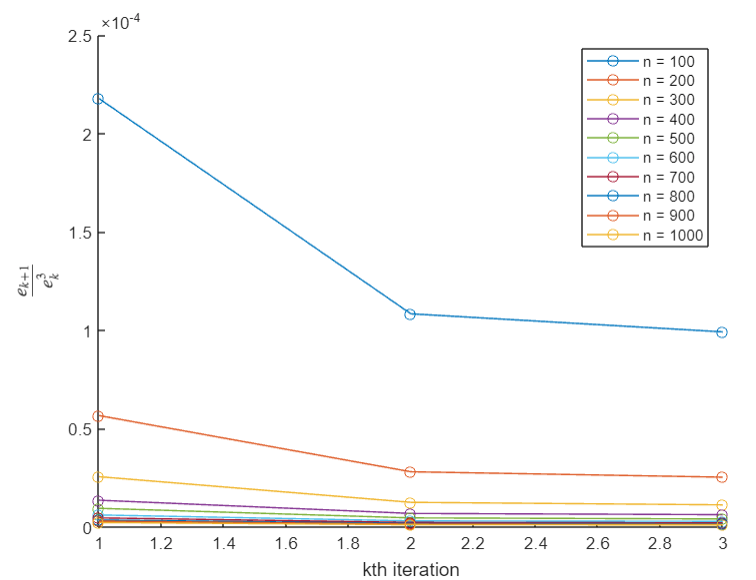
\includegraphics[width=0.8\textwidth,height=\textwidth,keepaspectratio]{lotsofplots.png}
        \caption{Plotting the error from the Rayleigh Quotient $e_{k+1}/e^3_k$ for matrix $A$ of size $n \times n$ where $n = 100^i$ for $i=[1,\dots,10]$.}
        \label{fig1}
    \end{figure}

\end{enumerate}

\end{proof}
\end{problem}






\end{document}